% Copyright 2020-2022 Robert Bosch GmbH

% Licensed under the Apache License, Version 2.0 (the "License");
% you may not use this file except in compliance with the License.
% You may obtain a copy of the License at

% http://www.apache.org/licenses/LICENSE-2.0

% Unless required by applicable law or agreed to in writing, software
% distributed under the License is distributed on an "AS IS" BASIS,
% WITHOUT WARRANTIES OR CONDITIONS OF ANY KIND, either express or implied.
% See the License for the specific language governing permissions and
% limitations under the License.

\hypertarget{description-robotframework-testcase-settings}{%
\section{\rfwcore\ Testcase Settings:}
\label{description-robotframework-testcase-settings}}

\begin{boxhint} {Hint}
  The below document is common for \rfwcore\ Testcase Settings before execution.
  So that, the generated *.xml result file will contains all required 
  information for importing to TestResultWebApp's database.\\
  \\
  However, we suppose to use \rfw\ with 
  \href{https://github.com/test-fullautomation/robotframework-testsuitesmanagement}{RobotFramework\_Testsuites}
  library for executing Robot testcase(s).

  It will help to define the below\rcode{Metadata}information implicitly within 
  the \rcode{Suite Setup} bases on your environment and configuration in *.json 
  file:
  \begin{itemize}
    \item \rcode{project}
    \item \rcode{version\_sw}
    \item \rcode{version\_hw}
    \item \rcode{version\_test}
    \item \rcode{machine}
    \item \rcode{tester}
    \item \rcode{testtool}
  \end{itemize}

  So that, you do not need to define these\rcode{Metadata}in your Robot test case.
\end{boxhint}

For the whole test execution:

\begin{itemize}

\item Project/Variant (can be overwritten by argument \rlog{--variant} or
  \rlog{--config} of
  \href{https://github.com/test-fullautomation/robotframework-robotlog2db}{\pkg}
  tool when importing):

\begin{robotcode}
Metadata    project     ${Project_name}
\end{robotcode}

\item Versions (can be overwritten by argument \rlog{--versions} or
  \rlog{--config} of
  \href{https://github.com/test-fullautomation/robotframework-robotlog2db}{\pkg}
  tool when importing):

\begin{robotcode}
Metadata    version_hw     ${Software_version}
Metadata    version_hw     ${Hardware_version}
Metadata    version_test   ${Test_version}
\end{robotcode}
\end{itemize}

For the Suite/File information:
\begin{itemize}

\item Description/Documentation:

\begin{robotcode}
Documentation   ${Suite_description}
\end{robotcode}

\item Author:

\begin{robotcode}
Metadata   author   ${Author_name}
\end{robotcode}

\item Component (can be overwritten by argument \rlog{--config} of
  \href{https://github.com/test-fullautomation/robotframework-robotlog2db}{\pkg} 
  tool when importing):
  
\begin{robotcode}
Metadata   component   ${Component_name}
\end{robotcode}

\item Test Tool - framework and python version, e.g \textbf{Robot Framework
  3.2rc2 (Python 3.9.0 on win32)}:

\begin{robotcode}
Metadata   testtool   ${Test_tool}
\end{robotcode}

\item Test Machine:

\begin{robotcode}
Metadata   machine   %{COMPUTERNAME}
\end{robotcode}

\item Tester:

\begin{robotcode}
Metadata   tester   %{USER}
\end{robotcode}

\end{itemize}

For test case information:

\begin{itemize}

\item Issue ID:

\begin{robotcode}
[Tags]   ISSUE-${ISSUE_ID}
\end{robotcode}

\item Testcase ID:

\begin{robotcode}
[Tags]   TCID-${TC_ID}
\end{robotcode}

\item Requirement ID:

\begin{robotcode}
[Tags]   FID-${REQ_ID}
\end{robotcode}
\end{itemize}


\hypertarget{description-sample-robotframework-testcase}{%
\section{Sample \rfwcore\ Testcase:}
\label{description-sample-robotframework-testcase}}

For test case management, we need some tracable information such as
version, testcase ID, component, ... to manage and track testcase(s) on
RQM.

So, this information can be provided in \rcode{Metadata} (for the whole
testsuite/execution info: version, build, ...) and \rcode{{[}Tags{]}}
information (for specific testcase info: component, testcase ID,
requirement ID, ...).

Sample \rfwcore\ testcase with the neccessary information for importing to
RQM:

\begin{robotcode}[caption=Sample \rfwcore\ testcase,
                  linebackgroundcolor=\hlcode{3,4,5,6,12,13,14}]
*** Settings ***
# Test execution level
Metadata   project        ROBFW              # Project/Variant
Metadata   version_sw     SW_VERSION_0.1     # Software version
Metadata   version_hw     HW_VERSION_0.1     # Hardware version
Metadata   version_test   TEST_VERSION_0.1   # Test version

# File/Suite level
Documentation             This is description for robot test file
Metadata    author        Tran Duy Ngoan (RBVH/ECM1)
Metadata    component     Import_Tools
Metadata    testtool      Robot Framework 3.2rc2 (Python 3.9.0 on win32)
Metadata    machine       %{COMPUTERNAME}
Metadata    tester        %{USER}

*** Test Cases ***
Testcase 01
   [Tags]   ISSUE-001   TCID-1001   FID-112   FID-111
   Log       This is Testcase 01

Testcase 02
   [Tags]   ISSUE-RTC-003   TCID-1002   FID-113
   Log       This is Testcase 01
\end{robotcode}

\begin{boxhint} {Hint}
Above highlighted\rcode{Metadata}definitions are not required when using \rfw.

\href{https://github.com/test-fullautomation/robotframework-testsuitesmanagement}{RobotFramework\_Testsuites}
library will handle these definitions within \rcode{Suite Setup}.
\end{boxhint}

\hypertarget{description-tool-features}{%
\section{Tool features:}\label{description-tool-features}}
\subsection{Usage:}
Please refer to \href{https://github.com/test-fullautomation/robotframework-robotlog2db#usage}{Usage section}
of package's repository or try with below command to get tools's usage:
\begin{robotlog}
RobotLog2DB -h
\end{robotlog}

The tool's usage should be showed as below:
\begin{robotlog}
usage: RobotLog2DB (RobotXMLResult to TestResultWebApp importer) [-h] [-v] 
                     [-recursive] [-dryrun] [-UUID UUID] [--variant VARIANT] 
                     [--versions VERSIONS] [--config CONFIG]
                     resultxmlfile server user password database

RobotLog2DB imports XML result files (default: output.xml) generated by the 
                     Robot Framework into a WebApp database.

positional arguments:
resultxmlfile        absolute or relative path to the result file or directory 
                     of result files to be imported.
server               server which hosts the database (IP or URL).
user                 user for database login.
password             password for database login.
database             database schema for database login.

optional arguments:
-h, --help           show this help message and exit
-v                   Version of the RobotLog2DB importer.
-recursive           if set, then the path is searched recursively for output 
                     files to be imported.
-dryrun              if set, then just show what would be done.
-UUID UUID           UUID used to identify the import and version ID on webapp. 
                     If not provided RobotLog2DB will generate a UUID for 
                     the whole import.
--variant VARIANT    variant name to be set for this import.
--versions VERSIONS  metadata: Versions (Software;Hardware;Test) to be set for 
                     this import (semicolon separated).
--config CONFIG      configuration json file for component mapping information.
\end{robotlog}

The below command is simple usage with all required arguments to import 
robot results into TestResultWebApp's database:
\begin{robotlog}
RobotLog2DB <resultxmlfile> <server> <user> <password> <database>
\end{robotlog}

Besides the executable file, you can also run tool as a Python module
\begin{robotlog}
python -m RobotLog2DB <resultxmlfile> <server> <user> <password> <database>
\end{robotlog}

\subsection{Handle missing information:}
\subsubsection{Default values:}
TestResultWebApp requires \rcode{Project}, \rcode{version_sw} to manage the 
execution results and \rcode{component} group test cases in the displayed charts.

In case above information is missing in \hyperref[description-robotframework-testcase-settings]
{testcase settings} during the test case execution, that leads to the 
missing information in the \emph{output.xml} result file.
So, these missing information will be set to default value when importing with
\href{https://github.com/test-fullautomation/robotframework-robotlog2db}{\pkg}
tool:

\begin{itemize}
\tightlist
\item \rlog{Project}: will be set to default value \pcode{ROBFW} if not defined.

\item \rlog{Software version}: will be set to execution time
  \pcode{\%Y\%m\%d\_\%H\%M\%S} as default value.

\item \rlog{Component}: will be set to default value \pcode{unknown} if not
  defined.
\end{itemize}

\subsubsection{Specify missing information with optional arguments:}
But, you can also provide the missing information as command arguments when executing the
\href{https://github.com/test-fullautomation/robotframework-robotlog2db}{\pkg}
tool with below optional arguments (refer its
\href{https://github.com/test-fullautomation/robotframework-robotlog2db\#usage}{usage}):

\begin{itemize}
\item \rlog{--variant VARIANT}

  To specify the {Project/Variant} information.

\item \rlog{--versions VERSIONS}

  To specify the {Software version} information.

\item \rlog{--config CONFIG}

  to provide a configuration \emph{*.json} file as \pcode{CONFIG} argument.
  Currently, the configuration \emph{*.json} supports 3 types of settings:

  \begin{itemize}
  \item \rcode{"version_sw"} to specify the \textbf{Software version} information as string value.
  \item \rcode{"variant"} to specify the \textbf{Project/Variant} as string value.
  \begin{boxwarning} {Warning:}
    These above settings will have lower priority than the commandline arguments
    \rlog{--variant VARIANT} and \rlog{--versions VERSIONS}
  \end{boxwarning}

  \item \rcode{"component"} to specify the \textbf{Component} information
        which will be displayed on
        \href{https://github.com/test-fullautomation/testresultwebapp}{TestResultWebApp}.
        Value can be:
        \begin{itemize}
          \item A string to apply a single \textbf{Component} or all test cases 
                within the execution result. E.g:
\begin{robotcode}
{
  "component" : "atest",
  ...
}
\end{robotcode}
          \item A json object to define the mapping between testcase folders and 
                \textbf{Components}. E.g:
\begin{robotcode}
  {
    "component" : {
      "cli"       : "robot/cli",
      "core"      : "robot/core",
      "external"  : "robot/external",
      "keywords"  : "robot/keywords",
      "libdoc"    : "robot/libdoc",
      ...
    },
    ...
  }
\end{robotcode}
        \end{itemize}
        The error will be occurred when the provided configuration
        \emph{*.json} schema is not correct.
  \end{itemize}
        

  Sample configuration json file:

\begin{pythoncode}
{
   "component"  : {
                  "cli"       : "robot/cli",
                  "core"      : "robot/core",
                  "external"  : "robot/external",
                  "keywords"  : "robot/keywords",
                  "libdoc"    : "robot/libdoc",
                  "output"    : "robot/output",
                  "parsing"   : "robot/parsing",
                  "reboot"    : "robot/reboot",
                  "rpa"       : "robot/rpa",
                  "running"   : "robot/running",
                  "std_lib"   : "robot/standard_libraries",
                  "tags"      : "robot/tags",
                  "test_lib"  : "robot/test_libraries",
                  "testdoc"   : "robot/testdoc",
                  "tidy"      : "robot/tidy",
                  "variables" : "robot/variables"
   },
   "version_sw" : "Atest",
   "variant"    : "ROBFW"
}
\end{pythoncode}
\end{itemize}


\newpage
\hypertarget{description-display-on-webapp}{%
\section{Display on WebApp:}\label{description-display-on-webapp}}

When the \emph{output.xml} file(s) is importing sucessfully to database,
the result for that execution will be available on
\href{https://github.com/test-fullautomation/testresultwebapp}{TestResultWebApp}.

Above settings in robot testcase will be reflect on \textbf{Dashboard}
(General view) and \textbf{Data table} (Detailed view) as below figures:

Execution result metadata:

\begin{figure}[h!]
  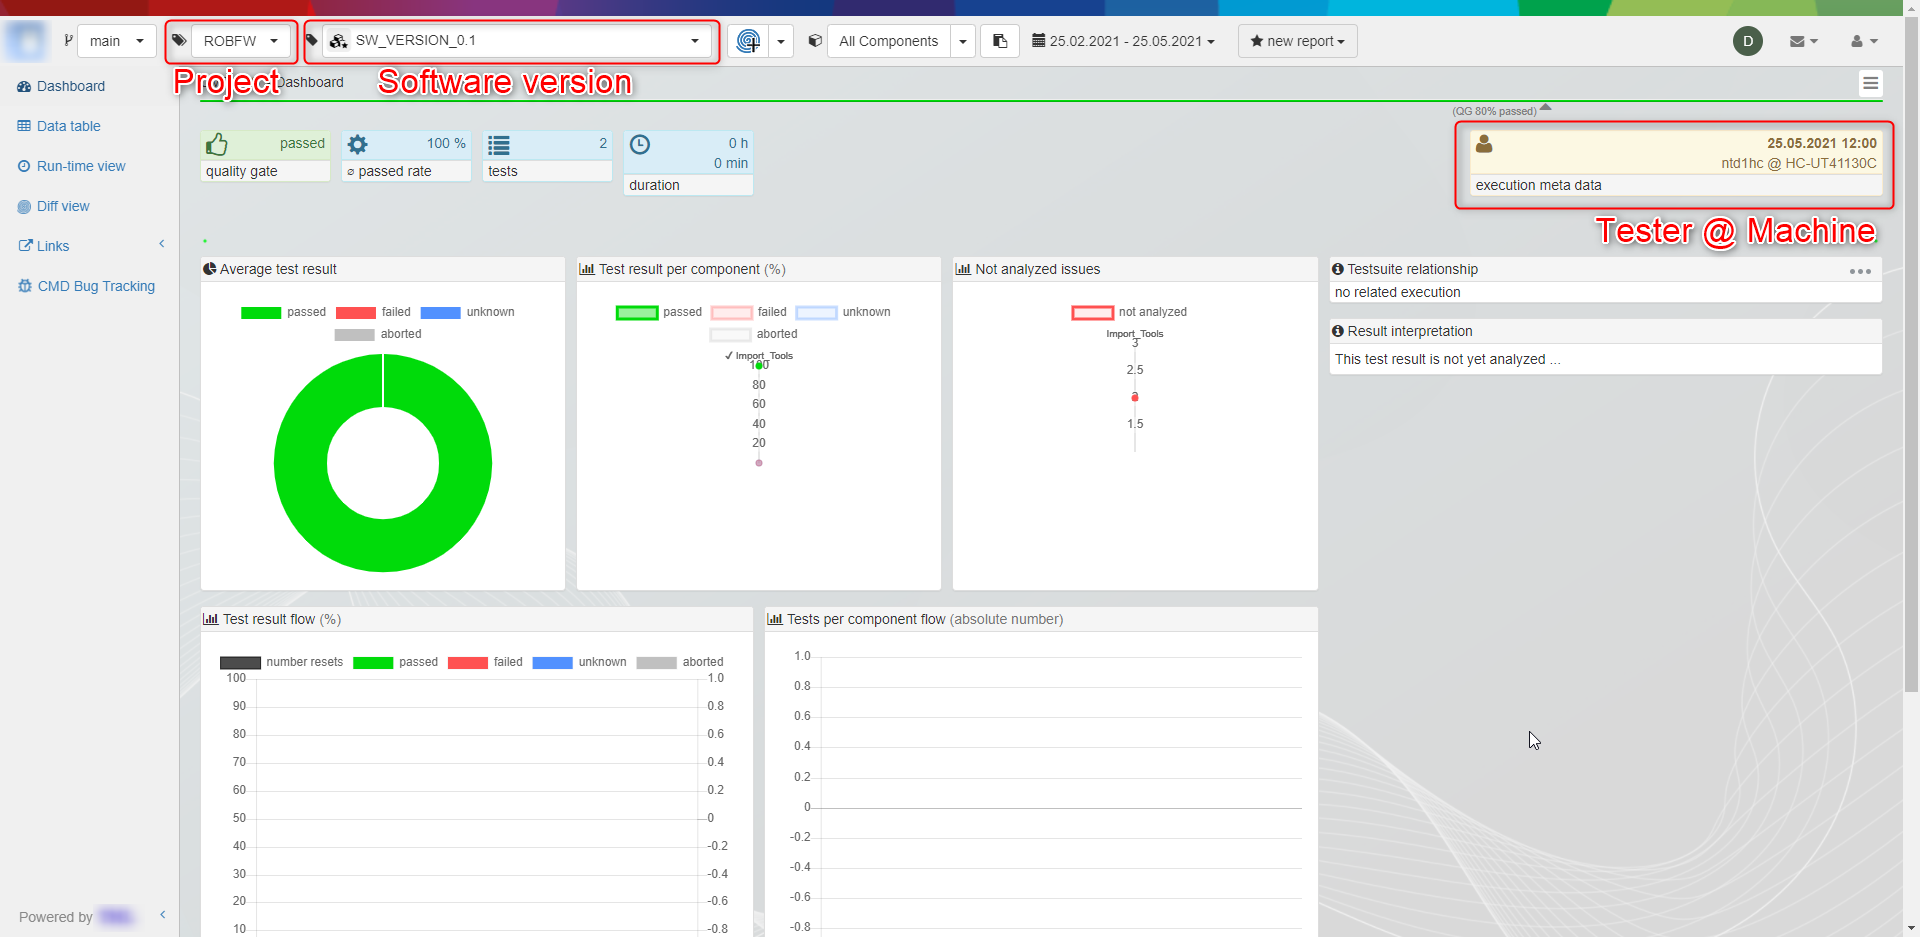
\includegraphics[width=1\linewidth]{./pictures/Dashboard.png}
  \caption{Dashboard view}
\end{figure}

Suite/File metadata and Testcase information:

\begin{figure}[h!]
  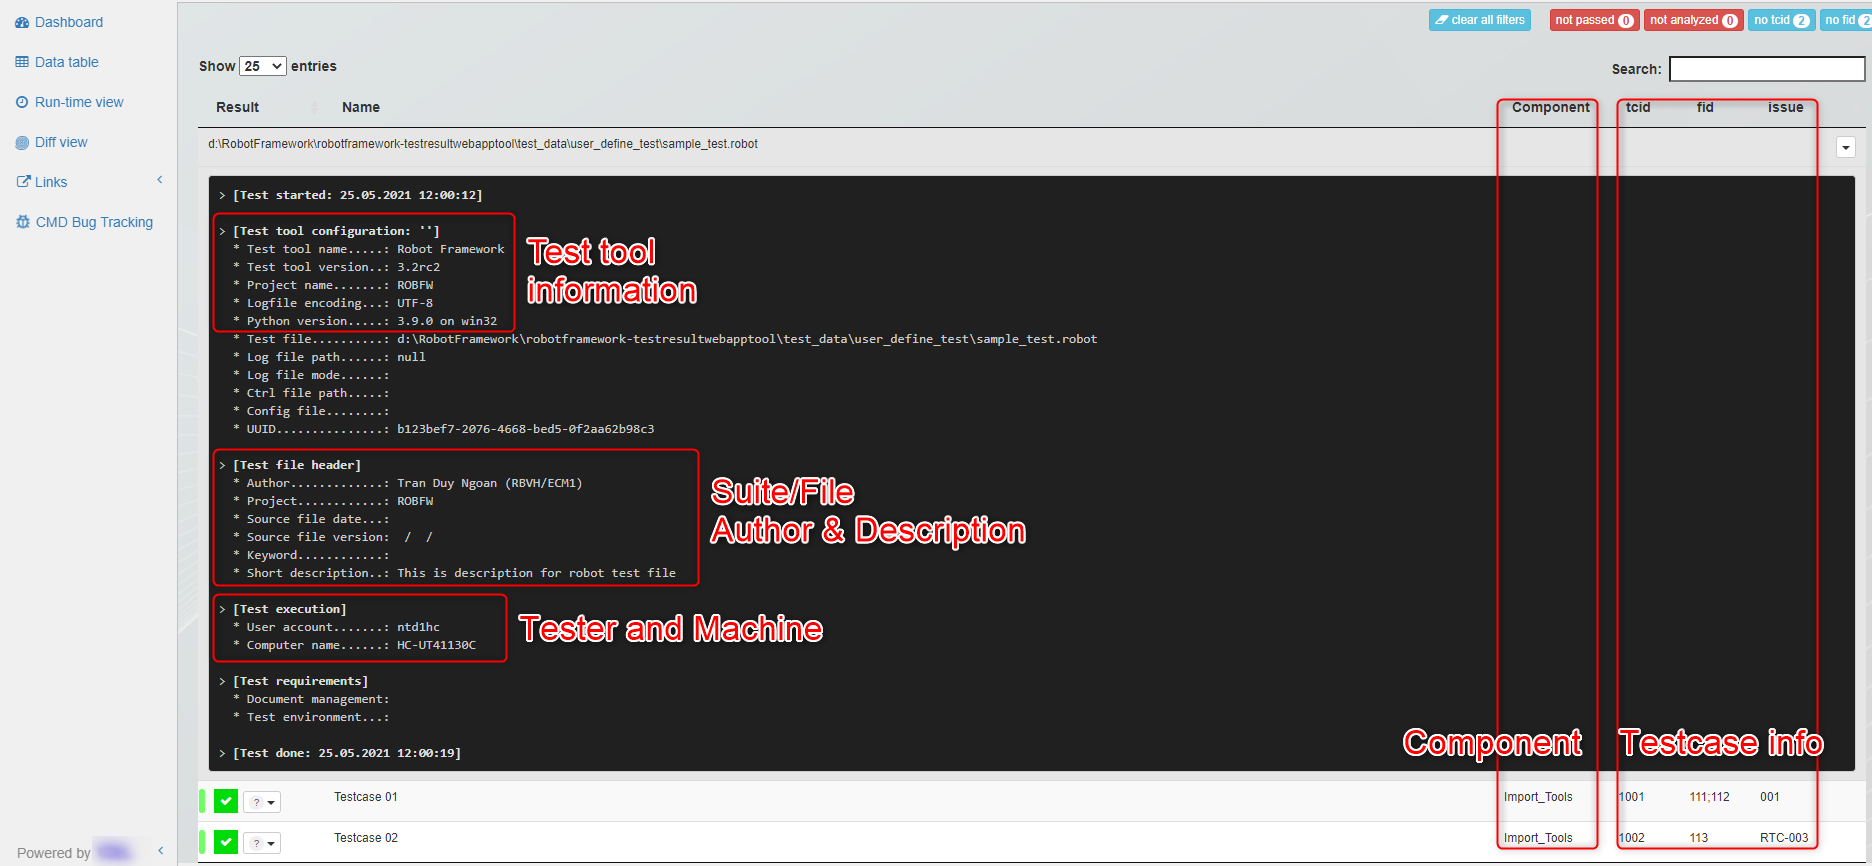
\includegraphics[width=1\linewidth]{./pictures/Datatable.png}
  \caption{Datatable view}
\end{figure}